\section{成员的属性}
\subsection*{静态成员}
一个类的非静态成员是无链接的。就以 \lstinline@valarri@ 为例,此对象的 \lstinline@_cap@ 成员和彼对象的 \lstinline@_cap@ 成员完全不是一个事物,它们在内存中有不同的地址——仅这一点足够说明问题了。\par
静态成员(Static member)则不然,它具有内部链接。换句话说,只要是这个类的静态成员,甭管是此对象的成员还是彼对象的成员,它们都是同一个事物,有完全相同的内存地址。
\begin{lstlisting}
struct C { //这里用struct是因为struct的成员访问权限默认为public,方便我们讲解
    int nonsta {}; //默认成员初始值
    static int sta;
};
int C::sta {}; //统一初始化为空,将初始化为0
int main() {
    C a,b;
    std::cout << &a.nonsta << std::endl << &a.sta << std::endl
        << &b.nonsta << std::endl << &b.sta << std::endl;
}
\end{lstlisting}
这段代码的输出结果为\\\noindent\rule{\linewidth}{.2pt}\texttt{
0x7ffd441a2908\\
0x600c54\\
0x7ffd441a290c\\
0x600c54
}\pagebreak
我们可以看到,这里 \lstinline@a.nonsta@ 和 \lstinline@b.nonsta@ 的地址值不同;而 \lstinline@a.sta@ 和 \lstinline@b.sta@ 的地址值相同。另外,读者也很容易注意到,静态成员的地址值与非静态成员的地址值也很不相同,这是因为它们的存储位置不一样——非静态对象的非静态成员位于栈段,而静态成员位于数据段或BSS段。\par
(非常量的)静态成员变量不能在类当中定义,只能声明;所以我们要把它放在类外定义,就像上面这段代码中写的那样。而在定义的时候呢,我们不能再写 \lstinline@static@ 了。\par
\lstinline@C::sta@ 定义在全局作用域,所以它不仅对于 \lstinline@C@ 类来说是静态成员,而且还具有外部链接——我们可以在一个源文件中为 \lstinline@C::sta@ 进行定义,而在另一源文件中不定义就可以使用它。
\begin{lstlisting}
//Header.hpp
struct C {
    static int sta; //静态成员变量
};

//Definition.cpp
#include "Header.hpp"
int C::sta {}; //它具有外部链接

//main.cpp
#include "Header.hpp"
int main() {
    std::cout << C::sta; //此C::sta与Definition.cpp中的C::sta一致
}
\end{lstlisting}\par
我们还可能会图方便,直接把 \lstinline@C::sta@ 定义在头文件中,但是我们会立刻发现一个问题:如果把 \lstinline@C::sta@ 定义在头文件中,那么两个源文件在包含此头文件后,就会在两个文件中分别产生两个定义,这就违反了单一定义规则(ODR),如图8.3所示。\par
\begin{figure}[htbp]
    \centering
    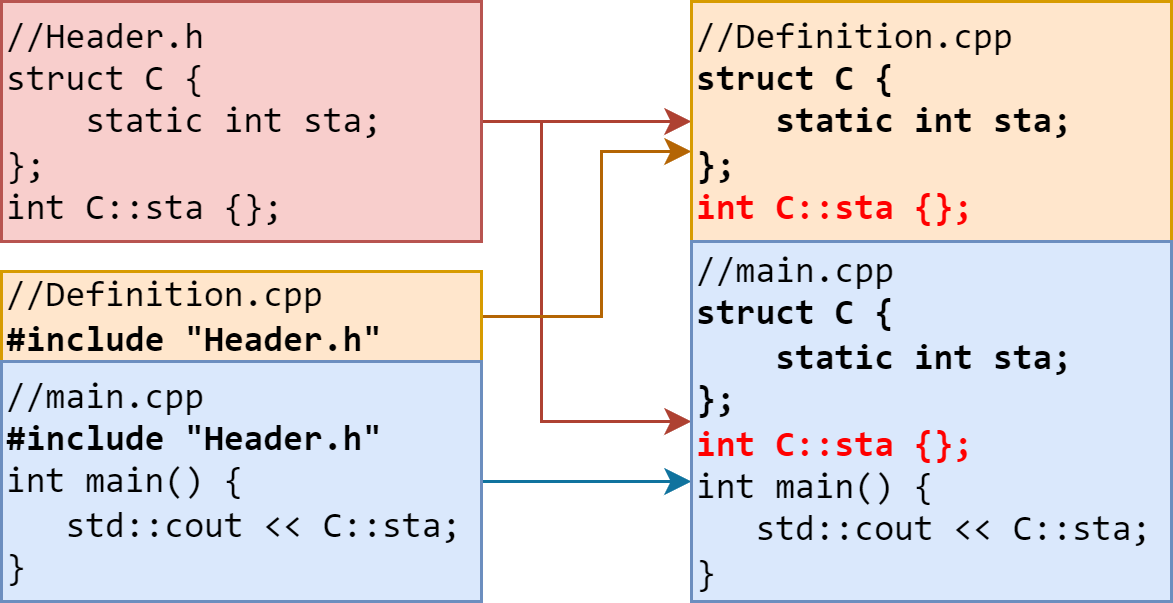
\includegraphics[width=\textwidth]{../images/generalized_parts/08_file_inclusion.drawio.png}
    \caption{把 \lstinline@C::sta@ 定义在头文件中将导致具有外部链接的变量被定义两次}
\end{figure}\pagebreak
所幸,从C++17起我们可以通过定义内联变量的方式来解决这个问题。
\begin{lstlisting}
//Header.hpp
struct C {
    static int sta;
}
inline int C::sta {};
\end{lstlisting}\par
\lstinline@inline@\footnote{关于 \lstinline@inline@ 的其它作用,有些资料声称使用 \lstinline@inline@ 可以降低部分函数运行的时间;而有些资料则声称不能。笔者在这方面无睱深入研究,所以本着宁缺勿滥的原则,不作此方面的介绍,仅介绍笔者已知的 \lstinline@inline@ 关键字作用。}关键字的作用在于,允许拥有外部链接的函数/变量在不同翻译单元中分别定义(但是,在每个翻译单元中仍然只能有单个定义)。这些定义应该要相同;如果不相同,编译器会自行选择其中一个作为它的定义(因为不能违反ODR)——那就属于未定义行为(Undefined behavior)了,我们最好别这么干。\par
对于定义在头文件的函数/对象来说,内联是我们的最佳选择。\par
言归正传。静态对象有很多用处,比如说在 \lstinline@valarray@ 类中,我们把 \lstinline@MAX_SIZE@ 成员定义成了静态成员。这样的好处在于,其一,它对 \lstinline@valarri@ 类的所有对象都是统一的,我们不必担心某个对象的数据被误修改从而导致不统一;其二,静态成员的内存空间是单独的,而且对于所有对象来说只此一个,这也就意味着我们不需要为每个对象都定义一个专属的 \lstinline@MAX_SIZE@ 成员,从而浪费大把的内存空间。\par
还有一个常见的应用是对象个数计数器。我们可以定义一个 \lstinline@_object_number@ 静态私有成员,它的初始值为 \lstinline@0@,可以在每个构造函数调用之时自增,而在每个析构函数调用之时自减。
\begin{lstlisting}
//声明
private:
    static std::size_t _object_number;
//定义
inline std::size_t valarri::_object_number {0};
\end{lstlisting}
至于构造函数和析构函数中相关的修改,我就不在此一一写出了。\par
虽然 \lstinline@_object_number@ 是私有成员,但是它也要在类外定义(静态成员的定义是唯一一个可以在类外``访问''私有对象的机会)。\par
我们还可以定义静态成员函数。静态成员函数虽然是成员函数,但是它没有 \lstinline@this@ 指针,也不能是常成员函数……总之有不少限制。但是我们可以直接用类名的形式来访问它,不需要用任何对象。
举个例子吧,我们可以定义静态成员函数 \lstinline@object_number@,让它返回 \lstinline@_object_number@ 静态成员变量。这样我们既能读取这个私有成员的值,又能防止外界对它的篡改。
\begin{lstlisting}
//声明&定义
public:
    static std::size_t object_number() { return _object_number; }
    //这个函数很短,直接定义就够了
\end{lstlisting}
这往后我们就可以用 \lstinline@valarri::object_number()@ 来返回当前有多少个 \lstinline@valarri@ 对象了。\par
\begin{lstlisting}
    std::cout << valarri::object_number();
\end{lstlisting}\par
\subsection*{常量成员}
我们可以把一个成员变量定义成常量成员变量——这个名字有点怪,我们就干脆叫它作``成员常量''好了。\par
一个成员常量一经初始化就不能再改了——这个初始化是初值列或默认成员初始值那样的初始化,而不是在构造函数体内部的那种看似``初始化''实则``赋值''的操作。我们在 \lstinline@valarri@ 类中定义过一个成员常量 \lstinline@MAX_SIZE@,实际上它还是一个静态成员。
\begin{lstlisting}
private:
    static const std::size_t MAX_SIZE {100000}; //MAX_SIZE是一个静态成员常量
\end{lstlisting}
对于静态成员来说,如果它是 \lstinline@const@ 或者 \lstinline@constexpr@,那么我们可以直接在类中给它定义,而不需要写在类外。\par
至于成员函数——我们可以定义常成员函数,但定义的方法是在参数列表和函数体之间的位置加上一个 \lstinline@const@。就以 \lstinline@valarri::size@ 为例,我们完全可以把它定义成常成员函数,这样写就好:
\begin{lstlisting}
//声明&定义
public:
    std::size_t size()const { return _size; } //返回当前的存储量大小
\end{lstlisting}
如果我们要把声明和定义分开写,那就需要在声明和定义处都写上这个 \lstinline@const@ 才行,一处也不能少。
\begin{lstlisting}
//声明
public:
    std::size_t size()const; //声明处要有const
//定义
std::size_t valarri::size()const { //定义处也要有const
    return _size;
}
\end{lstlisting}\par
说了半天,常成员函数到底是做什么的呢?我们又为什么要定义它呢?\par
不知读者是否有试过这样一种情形:
\begin{lstlisting}
void func(int &ref) {}//func函数接收一个引用,但它什么也不做
int main() {
    const int a {}; //把a定义成一个int型常量
    func(a); //试图把a作为实参传入func中
//error: binding reference of type 'int&' to 'const int' discards qualifiers
    return 0;
}
\end{lstlisting}
这个报错信息的含义是,不能把 \lstinline@int&@ 类型的形参绑定到 \lstinline@const int@ 类型的实参。\par
其实这是C++的一种防御机制,它不允许你把非常量的引用绑定到常量上;否则的话你就能够用这个引用来修改常量的值了,这成何体统啊?所以我们必须把 \lstinline@func@ 的参数设为 \lstinline@const int &ref@。只有这样,我们才能从函数声明上保证不用 \lstinline@ref@ 来修改其值;也只有这样,编译器才会放心地让我们像 \lstinline@func(a)@ 这样调用函数。\par
成员函数也是同理。读者应该记得我们说过,非静态成员函数都有一个隐藏参数,那就是``调用它的函数''。这个参数就像刚才的 \lstinline@func@ 一样,它把``调用它的函数''以一种类似引用的形式传入参数,所以我们可以通过 \lstinline@this@ 指针来改变此对象的成员(或者直接改变,这未必不是一种语法糖)。\par
但是如果我们需要定义一个常量对象呢\footnote{读者不要武断地认为,我们不需要用 \lstinline@const@ 定义常量对象,所以也不需要这些常成员函数之类花里胡哨的东西。不,我们需要!尤其是在引用参数传递时,只要你写成 \lstinline@const valarri&@,这时这个参数就会被当作常量对象!},这时我们就会发现问题了——
\begin{lstlisting}
    const valarri arr{1,2,3,4}; //定义一个常量对象
    std::cout << arr[0]; //试图访问arr[0],但我们没打算修改它的值
//error: passing 'const valarri' as 'this' argument discards qualifiers
\end{lstlisting}
这也同样是C++的保护机制在作怪——它不允许你把 \lstinline@arr@ 作为一个参数传给\\\lstinline@valarri::operator[](int)@,因为这个函数并不保证传入的隐藏参数是常量引用。\par
这也是是我们使用常成员函数的原因。当我们在参数列表之后加上一个 \lstinline@const@ 之后,我们就是在向编译器宣告:这个函数不会改变调用它的对象的值!
\begin{lstlisting}
//声明&定义
public:
    int& operator[](int i) { return _arr[i]; } //非常成员函数
    int operator[](int i)const { return _arr[i]; } //重载为常成员函数
\end{lstlisting}
这两个成员函数之间是重载关系。第一个函数接收一个隐藏的 \lstinline@valarri&@ 参数和一个 \lstinline@int@ 参数;第二个函数接收一个隐藏的 \lstinline@const valarri&@ 参数和一个 \lstinline@int@ 参数——所以它们是不一样的,编译器会有所选择\footnote{简单来说,编译器会对左值变量优先匹配 \lstinline@T&@ 参数,次优先匹配 \lstinline@const T&@ 参数;对左值常量优先匹配 \lstinline@const T&@ 参数,而不能匹配 \lstinline@T&@ 参数。我们在精讲篇中再谈。}。\par
读者还需要注意,这里第二个函数的返回类型不是 \lstinline@int&@ 而是 \lstinline@int@。这同样是防止修改常量的一种方式。只不过,如果我们不慎将它的返回类型真的定义成了引用,编译器也无法检查出来。如果在这种情况下``越狱''修改常量,那就会引发不可预知的后果,同样属于未定义行为。所以读者也勿必多留个心眼,不要在这里失误。\par
\lstinline@valarri@ 类中还有许多函数可以定为常成员函数,比如 \lstinline@valarri::max@, \lstinline@valarri::min@,\\\lstinline@valarri::sum@,还有 \lstinline@valarri::operator+(const valarri&)@ 之类的运算符,只要它们不需要修改 \lstinline@*this@ 本身,我们就可以把它们都定义成常成员函数——这样总是没有坏处的,毕竟可变对象可以调用常成员函数,但常量对象就真的不能调用非常成员函数(注意断句:非/常成员函数)了。
\begin{lstlisting}  
//声明
public:
    int sum()const; //总和
    valarri operator+(const valarri&)const; //可以与数组相加
    //其它几个省略
//定义
int valarri::sum()const { //返回值是当前数组中有效数据的总和
    int summation {0}; //先置为0
    for (int i = 0; i < _size; i++)
        summation += _arr[i]; //然后把每个数都加到summation上
    return summation;
}
valarri valarri::operator+(const valarri &a)const {
    valarri v; //有了默认构造函数之后可以不写花括号了
    v._cap = std::min(_cap, a._cap); //先确定v的容量
    v._arr = new int[v._cap]; //分配动态内存。_arr原本指向空,不用回收什么
    for (v._size; v._size<v._cap; v._size++)
        v._arr[v._size] = _arr[v._size] + a._arr[v._size];
    return v; //返回值是v
}
//其它几个省略
\end{lstlisting}
\subsection*{插曲——常量对象的指针成员}
一个类的对象可以用 \lstinline@const@ 限定符规定为常量对象。对于一个常量对象来说,它的基本数据类型成员变量——如 \lstinline@int@ 或 \lstinline@double@ 成员,都会变成 \lstinline@const@ 成员;它的数组会变成常量数组,我们不能用下标运算符改变数组的元素;它的指针会变成常量指针,即它的指向不能改变,但它的内容依旧可以改变。\par
常量指针是一个坑,我们需要在写代码时就加以防范,避免让这个类提供可以改变常量成员的途径,比如说在定义 \lstinline@valarri::operator[](int)const@ 时不小心把返回类型写成 \lstinline@int@ 这样。\par
一般来说,我们用这种方式来防范就已经足够。只要我们审慎地检查每一个点,就不会出现这种问题;但读者还是可能会想,我为什么不把它设为指向常量的指针呢?这样我们不是就可以防止修改内容呢?\par
但是请麻烦读者作一个整体性的思考:如果我们定义的是非 \lstinline@const@ 对象,那么我们应当允许这个指针没有限制地修改指向和内容;而如果我们定义的是 \lstinline@const@ 对象,那么我们应当禁止这个指针修改指向或内容。现在的困难是,如果我们定义了无任何限制的指针,那么常量对象的指针就能够修改内容;如果我们定义了指向常量的指针,那么非常量对象的指针也不能修改内容了!所以这种一刀切的方法是行不通的,无论怎样都会违背我们的初衷。\par
要正确地解决这个问题,我们的的原始思路是——定义两个指针,一个是无限制指针 \lstinline@_arr_m@;一个是指向常量的指针 \lstinline@_arr_c@。
\begin{lstlisting}
private:
    int *_arr_m; //指向变量的指针
    const int *_arr_c; //指向常量的指针
\end{lstlisting}
接下来,凡是在常成员函数中,我们就使用 \lstinline@_arr_c@;凡是在非常成员函数中,我们就使用 \lstinline@_arr_m@。另外需要注意,非常成员函数有可能会改变 \lstinline@_arr_m@ 的指向(比如说重新分配动态内存),所以我们每次改变 \lstinline@_arr_m@ 的地址值后都要把 \lstinline@_arr_c@ 和它的值对齐——也就是给 \lstinline@_arr_c@ 赋值为 \lstinline@_arr_m@ 的值\footnote{这个对齐操作不是一个建议,而是必须的。因为一个变量可以隐式类型转换成常量,所以对于变量对象来说,\lstinline@_arr_c@ 可能在此时用不到,但在彼时常量类型转换之后就可能用到了,不能弃之不顾。}。\par
这种做法有两项缺陷:第一,我们需要用两个指针来操作,不仅麻烦,还增加了内存占用(原来我们只需要一个指针就够);第二,我们总是要在改变 \lstinline@_arr_m@ 之后进行对齐,但这也是很容易被忘记的!其实它们的共同原因是,我们使用了两个指针;所以我们需要想到一种更有效,更方便,也更安全的方式。我的选择是:
\begin{lstlisting}
private: //valarri的private部分
    class Arr{ //内嵌的类,类名为Arr
    public:
        int*& p() {return _p;} //返回类型是“对指针的引用”
        const int* p()const {return _p;} //返回类型是“指向常量的指针”
    private:
        int *_p;
    }_arr; //直接定义该类的_arr对象
\end{lstlisting}\par
这种方法的特点在于,我们只需要一个 \lstinline@_arr._p@ 指针就可以了,既能节省内存空间,又不需要考虑对齐问题。\par
如果一个 \lstinline@valarri@ 对象是常量,那么它的成员 \lstinline@_arr@ 也是常量,所以每次调用 \lstinline@_arr.p()@ 的时候调用的都是它的常成员函数,返回值是指向常量的指针。这个返回值不是对指针的引用,所以它不能修改 \lstinline@_arr._p@ 的指向;同时它也不能修改内容,因为返回类型就是指向常量的指针。\par
如果一个 \lstinline@valarri@ 对象不是常量呢?那么它的成员 \lstinline@_arr@ 也不是常量,所以每次调用 \lstinline@_arr.p()@ 的时候调用的都是它的非常成员函数,返回值是对指针的引用。这个返回值是对指针的引用,所以它能修改 \lstinline@_arr._p@ 的指向;同时它也能修改内容。\par
再补充一些内容——为了方便用初值列或默认成员初始值,我们需要为 \lstinline@valarri::Arr@ 类设计一个构造函数。所以我们可以把它改成这样:
\begin{lstlisting}
    class Arr{ //内嵌的类,类名为Arr
    public:
        Arr(int *ptr) : _p{ptr} {} //构造函数,接收一个指针初始化
        int*& p() { return _p; } //返回类型是“对指针的引用”
        const int* p()const { return _p; } //返回类型是“指向常量的指针”
    private:
        int *_p;
    }_arr {new int[_cap]};
    //声明_arr时使用它的构造函数Arr::Arr(int*),这也是_arr的默认成员初始值
\end{lstlisting}
这个内嵌类对象的构造过程对于初学者来说,可能有点复杂,但是也不要太害怕,其中的道理还是我们前面讲的那些,只是在具体应用上,我们增加了一个嵌套,仅此而已。\par
接下来我们只需要在 \lstinline@valarri@ 所有成员函数中都使用 \lstinline@_arr.p()@ 就可以了,以下是一组例子:
\begin{lstlisting}
public:
    int& operator[](int i) { return _arr.p()[i]; } //非常成员函数
    int operator[](int i)const { return _arr.p()[i]; } //重载为常成员函数
\end{lstlisting}
这里的 \lstinline@_arr.p()[i]@ 表示方式看上去有点怪,但是我一解释你就懂了:\lstinline@_arr@ 是什么?它是一个 \lstinline@valarri::Arr@ 类的对象嘛。\lstinline@_arr.p()@ 是什么?它是 \lstinline@_arr@ 调用的成员函数嘛。\lstinline@_arr.p()@ 的返回值是什么?\lstinline@int*@ 或者 \lstinline@const int*@,总之是一个指针——实际上它会指向动态内存空间,也就可以作为动态数组使用。既然 \lstinline@_arr.p()@ 它是一个指针,那么我们用 \lstinline@_arr.p()[i]@ 来访问内容不就很合理吗?\par
\subsection*{\texttt{mutable}成员}
对于任何一个常量对象来说,它的非静态成员都会成为常量。这也就意味着,一经初始化,这个对象的任何值都不能进行修改了。\par
不过,在有些情况下,出于记录、标记等需要,即便一个对象是常量,我们也希望修改它的个别成员。\lstinline@mutable@ 关键字的作用在于,它强制规定了无论这个对象是不是 \lstinline@const@ 常量,这个成员都是可变的。\par
先举个简单的例子:我们需要一个计数器,来记录每一个对象调用某成员函数的次数。常量成员当然可以调用常成员函数,所以我们的计数器也需要可以改动。这时候使用 \lstinline@mutable@ 就合情合理了。
\begin{lstlisting}
class C {
public:
    void fun() { //非常成员对象版本
        ++count;
        //...
    }
    void fun()const { //常成员对象版本
        ++count; //计数器自增
        //...
    }
private:
    //...其它非mutable成员
    mutable std::size_t count; //计数器,即便对于常量对象来说也可变
};
\end{lstlisting}\par
还有一个更复杂的例子,就是作为\textbf{延迟标记(Lazy tag)}。
\subsubsection*{延迟标记}
在实际编程的过程中我们可能会遇到这样的问题:
\begin{lstlisting}
    char str1[10000] {/*太长,省略*/}, str2[10000];
    for (int i = 0; i < std::strlen(str1); i++)
        str2[i] = str1[i];
\end{lstlisting}
这段代码的运行效率很低,但我们不应该把它归咎于赋值语句;真正的问题出在 \lstinline@std::strlen@ 上。\lstinline@std::strlen@ 的算法原理是很原始的``逐个读取字符,直到遇到 \lstinline@'\0'@ 为止''。下面是它的一种可能的实现方式:
\begin{lstlisting}
std::size_t strlen(const char *start) {
    const char *end = start;
    while (*end != '\0')
        ++end;
    return end - start;
}
\end{lstlisting}
换句话说,我们每次调用 \lstinline@std::strlen(str1)@ 时,都是在逐个读取 \lstinline@str1@ 中的数据,最后计算出值来。那么这样的调用进行了多少次呢?\lstinline@std::strlen(str1)@ 次!如果这个字符串长达8000字节,程序将进行$8'000^2=64'000'000$次读取——相比之下,它只不过进行了8000次 \lstinline@str2[i]=str1[i]@ 的赋值而已。\par
但是我们想一下就会发现,这8000次调用的结果值都是一样的,所以我们完全没必要让它一遍遍地重新计算,直接计算一次,然后把这个值记录下来就好了。
\begin{lstlisting}
    char str1[1000] {/*太长,省略*/}, str2[1000];
    std::size_t str1len{ std::strlen(str1) }; //只调用std::strlen一次
    for (int i = 0; i < str1len; i++)
        str2[i] = str1[i];
\end{lstlisting}
这就是一种原始的``耗费一些存储空间,从而换取更少的计算时间'' (用空间换时间)思想,或曰记忆化(Memoization)。如果一个什么东西需要我们反复计算,但多次计算出来的值都相同,那我们就别浪费宝贵的时间了,直接找个变量把它存起来就好。\par
\lstinline@std::string@ 有一个 \lstinline@length()@ 成员函数,它的返回值就是一个预先计算好,并单独存起来的数\footnote{我们在第六章第五节中有介绍过。},所以它不需要进行多余计算,就能节省很多时间。
\begin{lstlisting}
    std::string str {/*太长,省略*/};
    for (int i = 0; i < str.length(); i++) //放心用,效率很高!
        //...
\end{lstlisting}\par
延迟标记在这个基础上更进一步。它连一开始的那次计算都不做了,只是打一个``搁置再议''的标签而已。什么时候开始计算呢?等我们需要这个值的时候再算。这样的好处是,如果在这个对象的整个生存期内都不需要用到这个值,那我们岂不是连第一次的计算都省了?(图8.4)\par
\begin{figure}[htbp]
    \centering
    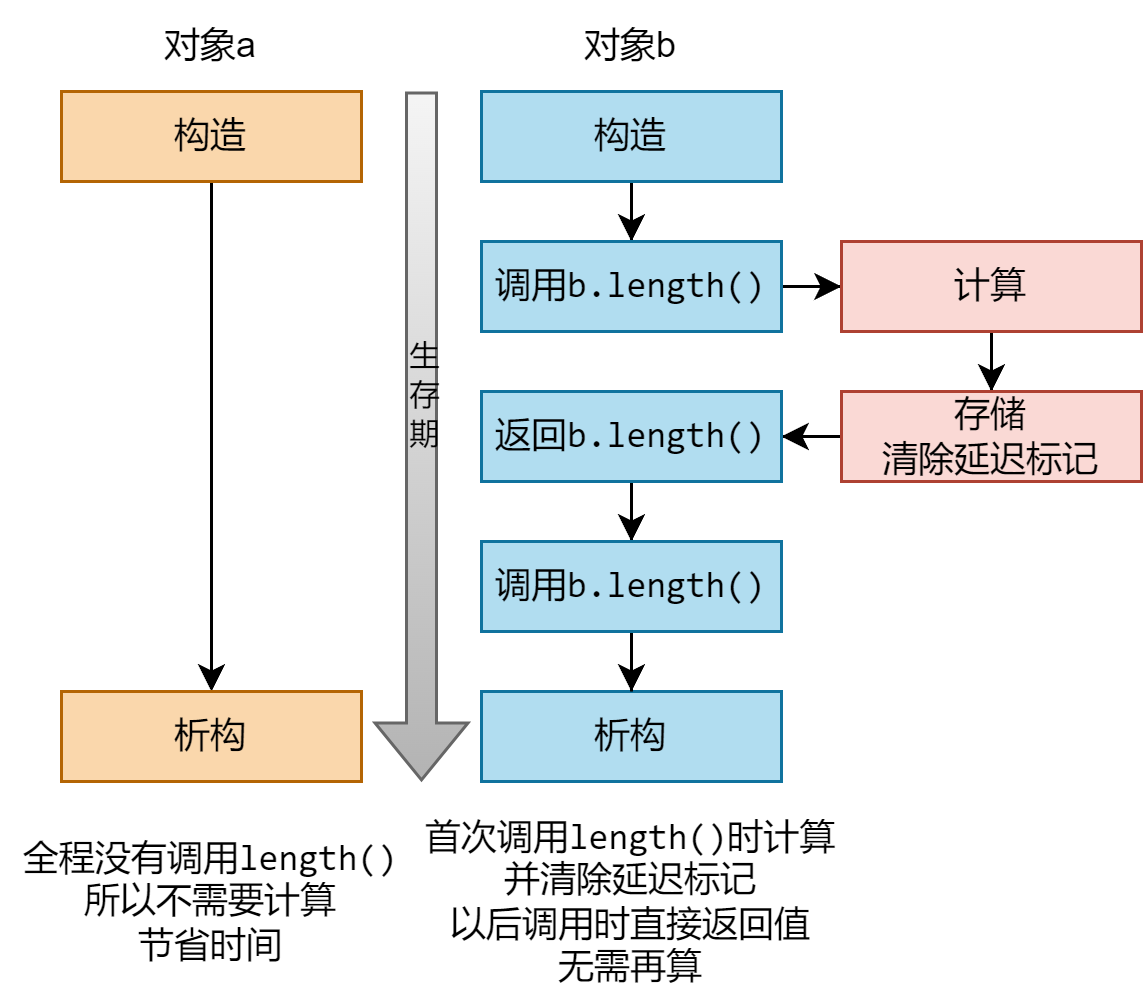
\includegraphics[width=.8\textwidth]{../images/generalized_parts/08_lazy_tag.drawio.png}
    \caption{延迟标记的作用}
\end{figure}
对于常量对象来说,我们为它设计的延迟标记也需要有修改的机会。就不拿 \lstinline@valarri@ 来举例了,我们换个例子。\par
一个三角形的三条边长$a, b, c$确定以后,我们就可以根据海伦公式计算出它的面积$A$:
\begin{align*}
s=&{}\frac12(a+b+c)\\
A=&{}\sqrt{s(s-a)(s-b)(s-c)}
\end{align*}
不过这个计算有点麻烦,我们可以提供一个延迟标记,等到需要这个值时再计算。
\begin{lstlisting}
#include <cmath>
class Triangle {
public:
    Triangle(double a, double b, double c)
        : _a {a}, _b {b}, _c {c} {} //函数体为空
    double area()const { //它是常成员函数,保证_a, _b, _c不会被修改
        if (!_area_cached) { //如果还没有缓存_area的值
            double s = (_a + _b + _c) / 2.; //临时变量s
            _area = std::sqrt(s * (s - _a) * (s - _b) * (s - _c));
            _area_cached = true; //现在它缓存了,延迟标记变为true
            //这两个mutable变量是可以在常成员函数中修改的
        }
        return _area; //返回已经缓存的面积值
    }
private:
    double _a;
    double _b;
    double _c;
    mutable bool _area_cached {false}; //延迟标记,false表示尚未缓存
    mutable double _area; //缓存的面积值
};
\end{lstlisting}\par
于是,当我们定义一个对象时,无论是不是常量对象,它都有这样的特点:
\begin{itemize}
    \item 如果一直不调用 \lstinline@area()@ 成员函数,这个值永远不会被计算,节省了计算时间;
    \item 第一次调用 \lstinline@area()@ 成员函数,这个值被计算出来并存储到 \lstinline@_area@ 中,与此同时延迟标记\linebreak\lstinline@_area_cached@ 消除;
    \item 以后再调用 \lstinline@area()@ 成员函数,直接返回 \lstinline@_area@ 就行了,无需再次计算。
\end{itemize}\par
很多人容易滥用 \lstinline@mutable@ 这个关键字,用来表达一些``可修改''的变量,然后把所有的对象都定义成 \lstinline@const@ 常量对象。这是非常糟糕的习惯!\par
\begin{lstlisting}
class Individual { //不要这样做!
private:
    std::string name;
    unsigned id;
    enum Sex : bool {male, female};
    Sex sex;
    mutable age; //年龄是可变的
};
const Individual /*定义各种对象都在用const*/;
\end{lstlisting}\par
而合理的用法应当是:当一个对象在逻辑上是不可变的时候(比如说,这个 \lstinline@Individual@ 对象的任何特性都一经定义就不发生变化),我们才会把它定义成常量对象。但如果只是个别成员不可变(比如姓名、身份号码),那我们应该把这些成员定为常量,而不是用常量对象+其它成员设为 \lstinline@mutable@ 的方式来实现。\par
那么在什么时候我们才会用 \lstinline@mutable@ 呢?应当是类似于上面那两种情况,即:这个成员与对象本身的逻辑关联并不大,它充当一个单独作用的量;但无论这个对象是否是常量,该成员都必须可变。这种情况是比较少见的,所以 \lstinline@mutable@ 在实际编程中出现的频率很低。\par
总而言之,\lstinline@mutable@ 是仅当我们有特殊需求的时候才会使用的,因此不要像刚才的例子那样滥用。\par
